L’architecture que nous avons proposée et les différents capteurs qui pourront être mis en place ont pour but d’aider le personnel médical dans le suivi de l’état de santé du patient. Nous allons détailler ici les différents services fournis à travers des applications destinées au personnel médical de l’hôpital. Ces différents services sont consultables sur la figure \ref{medical}.
\\
\begin{figure}[h!]
	\hspace*{-2.5cm}
	\centering
	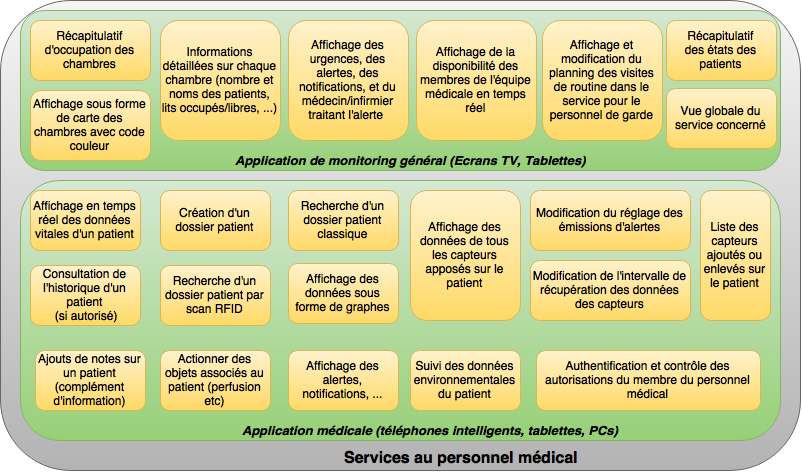
\includegraphics[width=1.4\textwidth]{medical.png}
	\caption{Services de la Couche Applicative du côté du Personnel Médical}
	\label{medical}
\end{figure}

Nous allons distinguer deux applications, l’une générale destinée au suivi des patients et du département de soins intensifs et la
seconde application qui permettra un suivi plus poussé du profil d’un patient en particulier. La figure \ref{appli} illustre cette
différenciation de services proposés en fonction de l'authentification. Nous allons détailler les différentes fonctionnalités de
la première application destinée au suivi général des patients du département. En effet, nous pouvons supposer qu’au niveau du
département de soins intensifs, il y a la présence d’une zone réservée au personnel d’astreinte où un service de gestion des
patients serait le bienvenu. Cette première application aura pour but d’aider le personnel médical dans la surveillance des
patients, et va donc permettre de centraliser certaines des différentes informations récupérées des différents capteurs et des
serveurs privés de l’hôpital. Cette première application sera destinée à un affichage sur des tablettes ou des écrans de télévision.  \\
\begin{figure}[h!]
	\hspace*{-2.5cm}
	\centering
	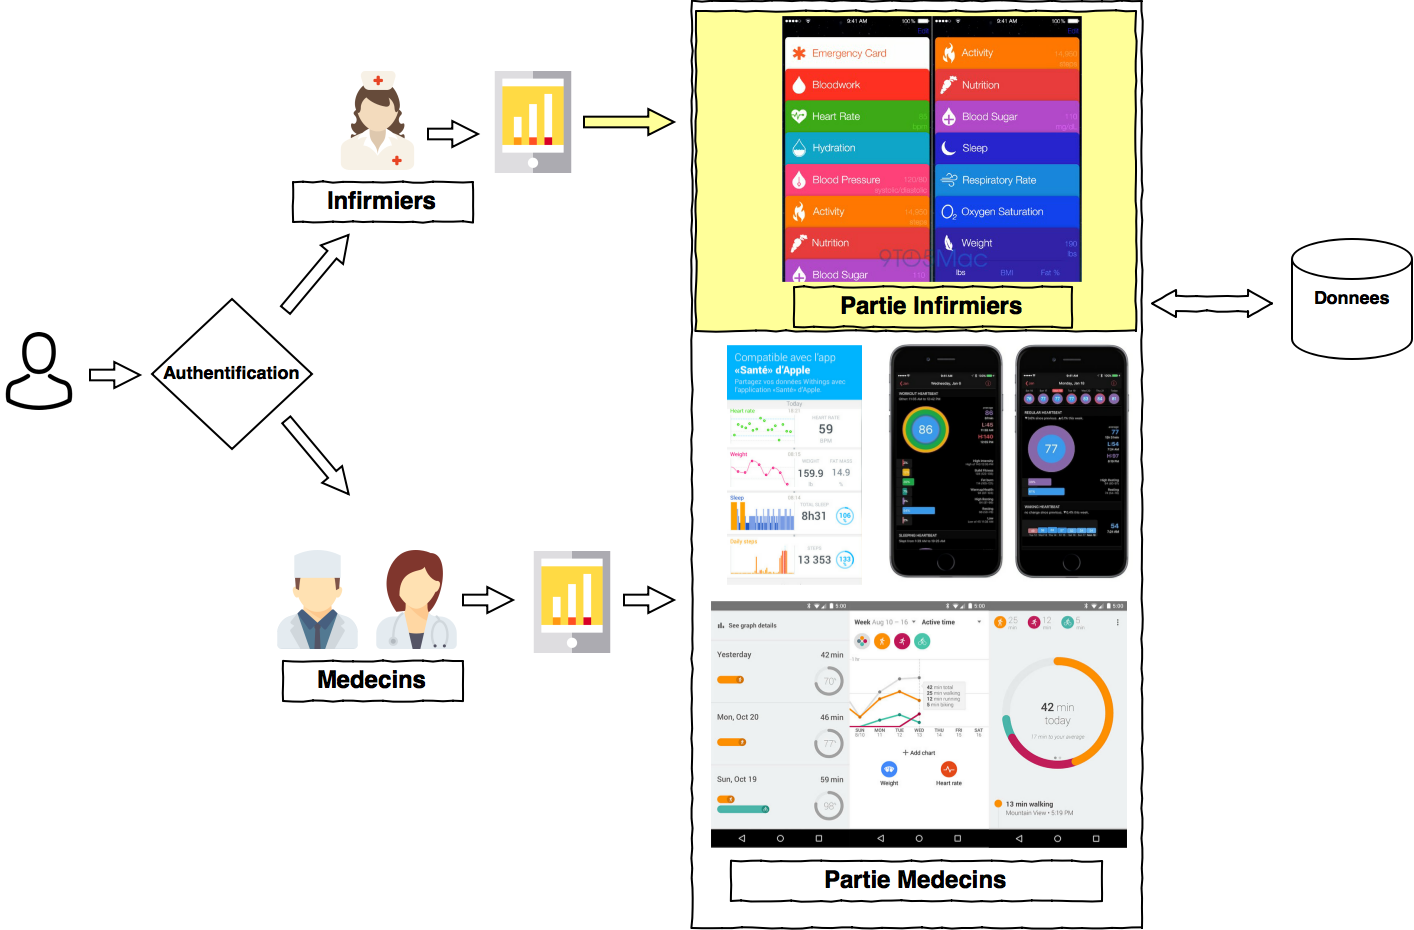
\includegraphics[width=1.4\textwidth]{Application.png}
	\caption{Différenciation des Services en fonction de l'Authentification du Personnel Médical}
	\label{appli}
\end{figure}

Pour intégrer les exigences de sécurité et de confidentialité que requiert le domaine médical, l’application contiendra un module
d’authentification qui assurera l’accès restreint aux données. Une fois l’authentification faite, l’application pourra être
utilisée de manière continue s’il n’y a pas de déconnexion ou d’interruption.


Une fois cette phase d’authentification faite, le ou les utilisateurs pourront accéder aux différentes données fournies par l’application provenant des capteurs et du Cloud. Par exemple, l’utilisateur pourra avoir accès aux différentes chambres, en sachant lesquelles sont occupées et lesquelles ne le sont pas.


L’application possédera ainsi une vue globale sur le département, avec la modélisation de l’occupation des chambres, l’état des différents patients présents dans le département de soins intensifs, et les informations générales permettant la surveillance du département.

Cette application aura la possibilité d’accéder à une page de consultation plus détaillée avec par exemple la possibilité d’avoir une vue sous forme de carte, sur laquelle un code couleur sera mis en place pour différencier les chambres occupées des chambres libres. L’application permettra d’accéder à des informations plus précises sur les chambres, avec la possibilité de connaître l’occupation des chambres, le nom des patients présents, les lits occupés ou libres. Et l’une des fonctionnalités principales de l’application sera la notification des alertes avec l’affichage des différents lits et chambres qui auraient émis une notification, une alerte ou une urgence. Lors de la réception d’une urgence ou d’un alerte, l’application affiche en plein écran la chambre et le lit d’où provient l’alerte. S’il y a plusieurs alertes qui sont émises, l’application fera alors un affichage sous forme d’une division de l’écran avec la présence d’une file pour pouvoir afficher toutes les alertes selon le niveau et l’ancienneté. Pour chaque alerte, lorsqu’un médecin confirme la prise en charge de l’urgence, l’affichage se complète pour signaler la mise à jour de la situation au reste du personnel médical.

Le personnel médical peut être informé en temps réel de la disponibilité et de l’activité de leur collègue. Cela permettra au chef de secteur de mieux organiser les ressources humaines à sa disposition et ainsi optimiser le traitement des patients.

Le personnel médical d’astreinte aura accès à une page de consultation des prochaines visites à faire avec les informations nécessaires au bon déroulement de ces visites de routines (affichage du numéro des chambres, du nom des patients,), l’application sera reliée au système de planification de l’hôpital. Il y a aura donc la possibilité d’accéder à un planning pour ajouter, modifier, supprimer des visites à faire pour les différents patients.
\\

La seconde application aura pour but d’aider le personnel médical à faire un suivi de manière plus précise d’un patient.

Pour intégrer les exigences de sécurité et de confidentialité que requiert le domaine médical, l’application contiendra aussi un module d’authentification qui assurera l’accès restreint aux données. Une fois l’authentification faite, l’application accédera au profil de l’utilisateur connecté pour connaître les droits que possède cette personne et afficher les différentes possibilités de navigation selon les droits qui ont été trouvés.

Une fois l’utilisateur authentifié, il pourra accéder aux différentes données fournies par l’application provenant des capteurs et
du Cloud. Les différentes données fournies par les capteurs placés sur le patient sont accessibles en temps réel, notamment pour
tout ce qui est suivi des signes vitaux, et au besoin l’application peut, si les droits de l’utilisateur le permettent, accéder
aux historiques des différentes données du patient.

L’utilisateur pourra ajouter un dossier patient, pour cela il lui suffira de rentrer certaines informations précises et définies en concordance avec les besoins du personnel médical. L’accès au profil utilisateur sera facilité par la présence des puces RFID d’identification des patients près du lit et dans le bracelet de celui-ci. Il suffira alors d’un simple scan d’une des deux puces. La recherche classique d’un profil du patient sera toujours possible selon différents critères. Une fois le profil affiché, les informations sur le patient sont consultables, et selon les informations dont le membre du personnel médical aurait besoin, il pourra naviguer de façon à voir les informations générales sur le patient ou des informations plus détaillées.

Au niveau des différentes informations auxquelles aura accès l’utilisateur, nous pouvons voir les différents éléments suivant ceux qui
proviennent des différents capteurs qui ont été proposés pour notre système. Il y a tout d’abord la possibilité d’accéder à
différentes informations vitales du patient comme le rythme cardiaque, la fréquence respiratoire, le rythme cardiaque, la
température du corps et la pression sanguine. Ces informations seront accessibles sous formes de graphes pour le suivi de l’état
de santé du patient. Les données des différents capteurs seront visibles à travers l’application, comme les données provenant du capteur pour la surveillance du cancer, ce qui permettra un suivi de l’évolution des différents indicateurs pour aider le diagnostic et le suivi du médecin, un accès au taux de glycémie du patient et son évolution, qui permettra ainsi au personnel médical d’injecter les bonnes doses d’insuline et permettre un suivi plus poussé de l’évolution de la glycémie, le suivi de l’activité cérébrale du patient sera aussi présent.

Le suivi de l’évolution des plaies sera aussi disponible grâce aux éventuels pansements intelligents mis en place sur le patient.
Le poids du patient pourra être surveillé, cet élément qui est un indicateur non vital, pourra permettre au personnel médical
d’avoir des renseignements supplémentaires quant à l’évolution de la santé du patient. Les mouvements des patients pourront être
suivis pour voir, notamment durant la phase de guérison, si le patient respecte bien ce qui a été indiqué par le personnel
médical. Par exemple, dans le cas où le patient doit restreindre ces mouvements, le personnel médical pourra savoir si ces
recommandations ont bien été suivies. Enfin les différentes données environnementales pourront être suivies pour notamment rassurer
les proches de la famille.

Aux différentes possibilités de consultation que l’utilisateur aura, s’ajoutera différentiations possibles sur les différents
éléments de l’environnement du patient. Il y aura la possibilité de modifier des paramètres de traitement des données sur le
patient, comme la possibilité de changer le temps d’émission des alertes, l’intervalle de temps entre la récupération de certaines
données depuis les capteurs, pour que le suivi puisse être vraiment propre à chacun des patients. Les paramètres de
traitement des données sur le patient et d’émission des alertes pourront être personnalisés pour pouvoir changer le temps
d’émission des alertes, l’intervalle de temps entre la récupération des données depuis les capteurs, le seuil d’émission des
alertes pour que le suivi soit le plus adapté possible au patient. L’application sera notifiée directement la mise en place ou le
retrait d’un nouveau dispositif par le personnel médical. 

Certains systèmes pourraient être directement contrôlés depuis l’application, comme le débit de la perfusion qui pourra être réglé à distance courte par le personnel médical. Pour ces fonctionnalités, une certaine sécurité sera mise en place en empêchant la modification si le membre du personnel médical n’est pas présent dans la pièce.

Les médecins et infirmiers pourront ajouter des notes au dossier du patient grâce à une fenêtre facilement accessible pour avoir un historique du suivi de l’état de santé du patient.

Cette application va permettre à l’utilisateur de recevoir les notifications d’alertes émises par les différents capteurs de
surveillance. Une fois que le médecin le plus adapté pour la gestion de l’alerte sera identifié par le système, un message sera
envoyé à travers le système pour le notifier  qu’une situation d’urgence a besoin de sa présence. Le médecin pourra alors notifier
de la prise en charge ou non de cette situation ce qui avertira le reste du personnel médical et permettra une meilleure gestion des ressources humaines du département.
